\documentclass{article}

\usepackage{amsmath, amsthm, amssymb, amsfonts}
\usepackage{thmtools}
\usepackage{graphicx}
\usepackage{setspace}
\usepackage{geometry}
\usepackage{float}
\usepackage{hyperref}
\usepackage[utf8]{inputenc}
\usepackage[english]{babel}
\usepackage{framed}
\usepackage[dvipsnames]{xcolor}
\usepackage{tcolorbox}

\colorlet{LightGray}{White!90!Periwinkle}
\colorlet{LightOrange}{Orange!15}
\colorlet{LightGreen}{Green!15}

\newcommand{\HRule}[1]{\rule{\linewidth}{#1}}

\declaretheoremstyle[name=Theorem,]{thmsty}
\declaretheorem[style=thmsty,numberwithin=section]{theorem}
\tcolorboxenvironment{theorem}{colback=LightGray}

\declaretheoremstyle[name=Proposition,]{prosty}
\declaretheorem[style=prosty,numberlike=theorem]{proposition}
\tcolorboxenvironment{proposition}{colback=LightOrange}

\declaretheoremstyle[name=Principle,]{prcpsty}
\declaretheorem[style=prcpsty,numberlike=theorem]{principle}
\tcolorboxenvironment{principle}{colback=LightGreen}

\setstretch{1.2}
\geometry{
    textheight=9in,
    textwidth=5.5in,
    top=1in,
    headheight=12pt,
    headsep=25pt,
    footskip=30pt
}

% ------------------------------------------------------------------------------

\begin{document}

% ------------------------------------------------------------------------------
% Cover Page and ToC
% ------------------------------------------------------------------------------

\title{ \normalsize \textsc{}
		\\ [2.0cm]
		\HRule{1.5pt} \\
		\LARGE \textbf{\uppercase{Journal #3}
		\HRule{2.0pt} \\ [0.6cm] \LARGE{Software defined networking} \vspace*{10\baselineskip}}
		}
\date{}
\author{\textbf{Mahsa Rahimian} \\ 
		University of Colorado/Colorado Springs\\
		09/11/2023 \\
		}

\maketitle
\newpage



% ------------------------------------------------------------------------------

\section{ “search” for survey papers/Gaps }

\begin{tex}
In this section, I will Critically/creatively read  five survey papers and write at 1/2 page of note. these notes will address some key elements of a survey paper and identify possible gaps in the survey. 

The first paper title is "Software defined networks: A survey"\cite{masoudi2016software}. the prpose of the paper is pretty clear which is to investigate SDN, its components, and the challenges it addresses. However, the abstract could be more concise.
the paper adequately sets the stage by explaining the context of SDN, mentioning the evolution of internet and ICT, and the challenges posed by traditional network management. However, it doesn't provide specific examples or data to support these claims. It successfully highlights the motivation for SDN by emphasizing its potential benefits in terms of flexibility and innovation opportunities. Still, it lacks specific examples of real-world applications or case studies that could strengthen this argument. the survey acknowledges the need for an overview of SDN but doesn't explicitly state what research gaps it intends to address. It mentions the investigation of data, control, and application planes, but it's not clear how this addresses existing gaps in the literature which I think it should be in this way since it is a survey paper and there isn't any expectation from a survey paper to talk about this subject. the paper discusses the challenges posed by traditional network management but does not provide specific examples or statistics to illustrate these challenges. Adding real-world scenarios would make the argument more compelling. it mentions challenges but does not delve into them in-depth. Exploring these challenges and potential solutions could be a valuable addition to the paper. also, The paper describes the state of the art and related works in the field of SDN but does not offer a comparative analysis of different approaches or technologies. Such a comparison could help readers understand the strengths and weaknesses of various SDN implementations.

the the second paper title is "State of the Art and Recent Research Advances in Software Defined Networking"\cite{bakhshi2017state}. this paper provides an overview of software-defined networking (SDN) and its historical context, emphasizing the need for SDN in addressing various challenges in networking. It discusses complementary technologies such as centralized network control, network programmability, and network virtualization, all of which have paved the way for the emergence of SDN.The introduction provides a clear and comprehensive overview of SDN and its significance in modern networking. It introduces the concept well, making it accessible to both experts and newcomers in the field. this survey The text discusses various supporting technologies such as centralized network control, network programmability, and network virtualization, which have influenced the development of SDN. This is crucial for understanding the foundation upon which SDN is built.the paper is The text is well-structured, with clear subsections that make it easy for readers to navigate and locate specific information.While this survey  briefly mentions the development of key technologies related to SDN, a more detailed comparative analysis of these technologies in terms of their strengths, weaknesses, and specific use cases would be beneficial. This would help readers understand why SDN emerged as the dominant paradigm. also, while the paper mentions that SDN encounters challenges in practical implementation, it doesn't delve into these challenges in depth. Providing examples and discussing real-world obstacles faced by SDN deployments would offer valuable insights to this survey. 

The third survey that was related to my research was "A survey on software defined networking with multiple controllers"\cite{zhang2018survey}. The introduction provides a clear explanation of SDN and its significance, emphasizing the decoupling of the control plane and data plane. It also highlights the challenges associated with a single controller in SDN networks.The paper outlines its objectives well, indicating that it aims to survey recent research on multiple controllers in SDN, discuss their benefits and challenges, and provide an overview of design principles, architectures, placement, and scheduling.The paper is structured in a logical and organized manner, with clear section headings and a well-defined flow of topics, making it easy for readers to follow the content.While the paper introduces SDN and its fundamental concepts, it could benefit from a more detailed explanation of SDN's evolution and why it's necessary. Providing examples of real-world problems that SDN addresses would make the introduction more engaging and informative. the survey mentions that multiple controllers are required in many scenarios but does not elaborate on these scenarios or provide specific use cases. Including real-world examples of network deployments that benefit from multiple controllers would make the content more practical.

the fourth paper title is " Quality of Service (QoS) in Software Defined Networking (SDN): A survey"\cite{karakus2017quality}. The paper identifies that QoS support in traditional networking architectures is challenging. It introduces the concept of SDN and highlights its advantages for QoS provisioning, such as centralization, programmability, and separation of the data plane and control plane. The paper categorizes various QoS-related mechanisms in SDN/OpenFlow networks, including multimedia flows routing, inter-domain routing, resource reservation, queue management, Quality of Experience (QoE)-aware mechanisms, network monitoring, and other QoS-centric mechanisms. It discusses the capabilities of OpenFlow protocol versions for QoS. The paper provides a broad overview of QoS in SDN/OpenFlow networks and categorizes various mechanisms, but it lacks in-depth analysis of each category. It doesn't delve into the specific challenges and solutions within each category.While the paper mentions the advantages of SDN for QoS, it does not provide real-world examples or case studies of SDN deployments that have successfully improved QoS. This practical perspective is essential to understand the feasibility and challenges of implementing QoS in SDN networks.
this paper is a highly cited paper. here is some of the reason that I think it cited more than 400 times. At the time of its publication, the paper addressed a pressing issue in networking, which was the need for improved QoS in the face of increasing network traffic diversity.The paper provides a comprehensive overview of QoS-related mechanisms in SDN/OpenFlow networks, making it a valuable resource for researchers and practitioners seeking to understand the field.The categorization of QoS mechanisms into different classes makes the paper structured and easy to navigate, catering to a wide audience.

The last paper that I would like to review is "Software Defined Networking: Research Issues, Challenges and Opportunities" \cite{mishra2017software}. The survey paper discusses the challenges, opportunities, and research issues in Software Defined Networking (SDN) and how to select the best SDN controller to reduce network complexity, implementation costs, and maintenance efforts in large organizations. The paper highlights the significance of SDN in addressing the limitations of traditional networking, such as separate control and data planes, lack of centralized visibility, and scalability issues. It emphasizes the need for a centralized controller to manage network devices efficiently.The paper acknowledges several challenges in SDN implementation, such as scalability, hardware and software requirements, technical resource allocation, traffic engineering, and network resiliency. These challenges create gaps in the existing SDN solutions.The survey recognizes the importance of making the underlying infrastructure layer vendor-independent. However, it doesn't delve into specific strategies or solutions to achieve this goal.Based on the gaps identified in the paper, here are some suggestions for a survey paper with novelty: in my opinion it should Conduct an in-depth analysis and comparison of various SDN controllers beyond what is briefly mentioned in the paper. Evaluate their features, performance, and suitability for different use cases. Identify emerging controllers or unique features that might not be widely recognized.also, it should dive deeper into SDN security mechanisms and present innovative approaches to securing SDN architectures. Discuss threat detection, mitigation, and compliance in SDN environments.
based on my review of four other papers that has lower citation, I think The paper may have low citations due to several reasons such as lack of In-depth analysis, limited practical guidance and lack of novelty. 
Here is the link:https://www.overleaf.com/project/64ff7d6d95836cc72bce46fd
\end{tex}
   




\subsection{Pictures }

\begin{figure}[htbp]
    \center
    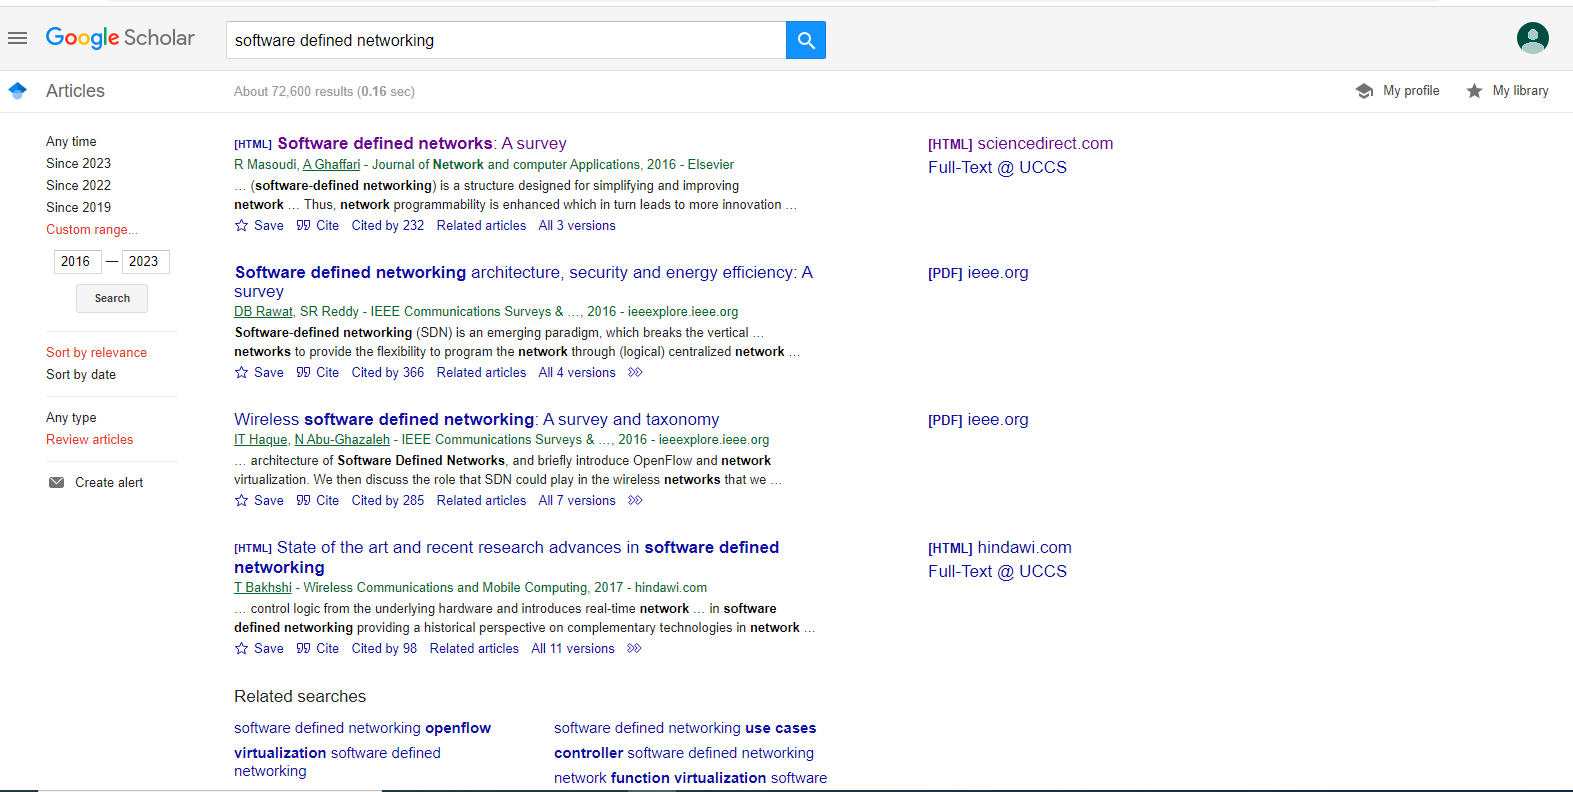
\includegraphics[scale=0.4]{screenshot.png}
    \caption{Screenshot of my search for survey papers on my topic}
\end{figure}






% ------------------------------------------------------------------------------
% Reference and Cited Works
% ------------------------------------------------------------------------------

\bibliographystyle{IEEEtran}
\bibliography{References.bib}

% ------------------------------------------------------------------------------

\end{document}
